\documentclass[11pt,a4paper]{article}
\usepackage[T1]{fontenc}
\usepackage[utf8]{inputenc}
\usepackage{lmodern}
\usepackage{microtype}
\usepackage[margin=2.1cm]{geometry}
\usepackage{booktabs}
\usepackage{graphicx}
\usepackage{float}
\usepackage{amsmath,amssymb}
\usepackage{xcolor}
\usepackage{enumitem}
\usepackage{caption}
\usepackage{adjustbox}
\usepackage{array}
\newcolumntype{L}[1]{>{\raggedright\arraybackslash}p{#1}}
\usepackage[colorlinks=true,linkcolor=blue!50!black,citecolor=blue!50!black,urlcolor=blue!50!black]{hyperref}
\setlist{nosep,leftmargin=1.3em}
\captionsetup{font=small,labelfont=bf}
\graphicspath{{../figures/}}
\newcommand{\tab}[1]{\input{tables/#1.tex}}
\newcommand{\todo}[1]{\textcolor{red!70!black}{[TODO: #1]}}
\IfFileExists{tables/val_automl.tex}{\newcommand{\nTrials}{34}\newcommand{\nComplete}{23}\newcommand{\nPruned}{11}\newcommand{\bestFamily}{Ridge least-squares}\newcommand{\bestCV}{0.9827}\newcommand{\bestTrial}{25}}{}

\title{\textbf{Phish or Not?}\\[2pt]\large Does a Phishing E-mail Detector Generalise to Unseen E-mail Sources?\\[4pt]
\normalsize Week 2 report: data analysis, learning plan, baseline, state of the art and AutoML v0.1}
\author{Imene Khelil \and Florian \and Ambroise \and Dylan\\[2pt]\small ESILV, Machine Learning 2026 (N.~Mellouli), major OCC}
\date{November 2026}

\begin{document}
\maketitle

\begin{abstract}
\noindent We study e-mail threat detection on the public \emph{Phishing Email Dataset} (82,486 e-mails pooled from six corpora collected between 1998 and 2022). Before modelling we audited the raw data and found three issues that published work on this dataset does not report:
(i) 13\% of the e-mails are exact or near-duplicates (including 3,919 copies of one 2008 malware campaign);
(ii) the source corpus can be predicted from the text with 98.7\% accuracy, so a classifier can learn \emph{where an e-mail comes from} instead of \emph{whether it is a scam};
(iii) the positive class mixes generic spam with phishing.
A plain TF-IDF + logistic regression baseline, trained on a de-duplicated, leakage-controlled split, reaches F1 = 0.991 in-distribution, on par with the published state of the art. When the test corpus is a source never seen in training, the false-positive rate rises from 0.9\% to 5--23\%, and only 59\% of modern (2015--2022) phishing e-mails are detected. Our numbers reproduce the leave-one-corpus-out results of Bhuiyan \& Bhuiyan (2026) to within 0.05 F1. An AutoML v0.1 pipeline (Optuna, 6 model families, selection on in-distribution CV) picks a more complex model. That model lowers the in-distribution FPR (0.65\%) but generalises \emph{worse} than the baseline on three of four unseen sources. This shows that the model-selection criterion, not the model family, is the bottleneck, and it defines the work plan for v0.2+.
\end{abstract}

%=====================================================================
\section{Business scope}
E-mail remains the main initial-access vector for attacks on organisations and connected-object fleets (credential theft, malware droppers, fake invoices). A detector is useful only if it keeps working \emph{on mail it was not trained on}: new organisations, new campaigns, new years. Two error types have very different costs:
a missed phishing e-mail (false negative) can compromise an account, while a quarantined legitimate e-mail (false positive) costs user time and trust, and because malicious mail is a small fraction of real traffic, even a few percent of false positives can drown the real alerts.

\textbf{Objective.} Build a text-based classifier \emph{spam/phishing vs legitimate} and measure honestly how well it transfers to an unseen e-mail source. \textbf{Link to the OCC major:} threat detection on communication channels, robustness of a security model under distribution shift, and adversarial thinking (shortcut features are exactly what an attacker can evade).

%=====================================================================
\section{Problem formalisation}
Each e-mail $i$ is the text $x_i$ = subject + body, with label $y_i\in\{0,1\}$ (1 = spam or phishing). We learn $f:x\mapsto \hat p(y{=}1\mid x)$ and predict $\hat y = \mathbb{1}[\hat p \ge 0.5]$.
Each e-mail also has a source $s_i\in\{$CEAS\_08, Enron, Ling, Nazario, Nigerian\_Fraud, SpamAssasin$\}$, used \emph{only} to build evaluation splits, never as a feature (it is not available at deployment).

\textbf{Two evaluation regimes.}
(1) \emph{In-distribution}: random hold-out test drawn from the same mix of sources as training.
(2) \emph{Out-of-distribution (LOSO, leave-one-source-out)}: train on five sources, test on the sixth.

\textbf{Metrics.} Precision, recall and F1 of the malicious class; false-positive rate $\mathrm{FPR}=FP/(FP+TN)$; ROC-AUC and PR-AUC; Brier score for probability calibration. Because the pooled dataset is 48\% malicious while real traffic is not, we also report the precision the same classifier would have at a prevalence $\pi$ (TPR and FPR do not depend on prevalence):
\begin{equation}
\mathrm{Prec}_\pi = \frac{\mathrm{TPR}\,\pi}{\mathrm{TPR}\,\pi + \mathrm{FPR}\,(1-\pi)}, \qquad \text{reported at } \pi = 5\%.
\end{equation}
Accuracy is shown only for reference, never used for decisions.

%=====================================================================
\section{Dataset description, source and suitability}\label{sec:dataset}
\subsection{Source and access}
\begingroup\sloppy
\begin{itemize}
\item \textbf{Dataset:} \emph{Phishing Email Dataset} (``Phish No More: The Enron, Ling, CEAS, Nazario, Nigerian \& SpamAssassin Datasets''), published on Kaggle by N.~A.~Alam, one of the authors of \cite{alsubaiey2024}: \url{https://www.kaggle.com/datasets/naserabdullahalam/phishing-email-dataset}. Last updated 24 May 2024; 7 CSV files, 261~MB. The Kaggle page asks users to cite \cite{alsubaiey2024}.
\item \textbf{Category (guidelines):} public dataset (Kaggle) built from \emph{scientific datasets published with research papers}. The same per-source CSVs are archived on Zenodo by Champa, Rabbi \& Zibran \cite{champa_zenodo}.
\item \textbf{Files used:} the six per-source files (\texttt{CEAS\_08.csv}, \texttt{Enron.csv}, \texttt{Ling.csv}, \texttt{Nazario.csv}, \texttt{Nigerian\_Fraud.csv}, \texttt{SpamAssasin.csv}), not the pre-merged \texttt{phishing\_email.csv}: the merged file has no source column and its text was already transformed by the authors (AI\_AUDIT \#5).
\item \textbf{Acquisition and integrity:} our working environment could not reach Kaggle, so the files were retrieved from a public GitHub mirror of the same package. Row counts and label counts match the published totals exactly (82,486 e-mails; 42,891 label 1; 39,595 label 0), and so do the per-corpus sizes reported by \cite{bhuiyan2026}. SHA-256 hashes are listed in \path{data/README.md}. \todo{each member re-downloads from Kaggle and checks the hashes}
\end{itemize}
\endgroup

\subsection{Observations, features, data type and labels}
\begin{itemize}
\item \textbf{Observations:} 82,486 e-mails (71,386 after de-duplication, Section~\ref{sec:dup}).
\item \textbf{Features:} unstructured \textbf{text} (\texttt{subject}, \texttt{body}) for all sources. Four sources also have metadata: \texttt{sender}, \texttt{receiver}, \texttt{date} (strings) and \texttt{urls} (binary flag). Enron and Ling have only subject + body. The model therefore works on text; numerical features (length, URL count, digit density, etc.) are \emph{derived} from it.
\item \textbf{Target:} binary \texttt{label} provided for every e-mail (1 = spam/phishing, 0 = legitimate), so the task is supervised classification with no labelling effort. The labels come from the original corpus curators (spam traps, personal phishing mailbox, manual ham/spam sorting) and their definition of ``spam'' differs between corpora.
\item \textbf{Extra variable:} the \texttt{source} corpus (added by us from the file name), which enables leave-one-source-out evaluation.
\end{itemize}

\subsection{Component corpora, licences and usage restrictions}
\begin{table}[H]\centering\small
\caption{The six component corpora. Licences were checked on the original distribution pages (November 2026); ``none found'' means no explicit licence could be located.}\label{tab:licences}
\begin{adjustbox}{max width=\linewidth}
\begin{tabular}{L{2.5cm}L{4.4cm}L{1.9cm}L{1.6cm}L{6.4cm}}
\toprule
Corpus & Origin & Period & Classes & Licence / terms of use \\
\midrule
CEAS\_08 & CEAS 2008 live spam-filter challenge (Univ.\ of Waterloo) & 2008 & ham, spam & None found; distributed as an academic research corpus, so we treat it as research-only and do not redistribute it. \\
Enron & Enron employees' mailboxes, released publicly during the FERC investigation; spam added by corpus curators & ham c.\ 2000--2002; spam later & ham, spam & None found for the labelled version; underlying e-mails are public record. Real people's names and messages: privacy-sensitive. \\
Ling & Ling-Spam: Linguist mailing list + spam & before 2001 & ham, spam & None found; research corpus. \\
Nazario & J.~Nazario's personal phishing mailbox (monkey.org) & 2015--2022 & phishing only & \textbf{CC BY 4.0} (\texttt{LICENSE.txt} on monkey.org): attribution required, changes must be indicated. \\
Nigerian\_Fraud & CLAIR collection of fraud e-mail (D.~Radev, ACL ADCR2008T001) & 1998--2007 & fraud only & \textbf{CC BY-SA 3.0 US}; citation of Radev (2008) required. \\
SpamAssassin & Apache SpamAssassin public corpus & 2002 & ham, spam & No formal licence. Copyright stays with the original senders; messages must never be sent into a live mail system; maintainer asks to be told of publications. \\
\midrule
\textbf{Kaggle package} & Merge of the six above & & & \textbf{CC BY-SA 4.0}; cite \cite{alsubaiey2024}. \\
\textbf{Zenodo mirror} & Champa et al.\ curated version & & & \textbf{CC BY 4.0}; cite Champa, Rabbi \& Zibran (ISDFS 2024, ICMI 2024). \\
\bottomrule
\end{tabular}
\end{adjustbox}
\end{table}
\textbf{How we comply.}
(1) Raw data is \emph{not} committed to the repository or the submission zip: \path{data/README.md} explains how to download it.
(2) Attribution: the Kaggle package, the Zenodo record and the CLAIR collection are cited.
(3) Share-alike: any derived dataset we publish (e.g.\ our de-duplicated corpus) would have to be released under CC BY-SA 4.0. We do not publish it.
(4) Privacy: we only show aggregate statistics and single tokens in the report, never full Enron e-mails. The names that appear in Table~\ref{tab:tokens} (e.g.\ \texttt{vince}, \texttt{kaminski}) are given only to show artefacts.
(5) SpamAssassin condition: no message is ever sent through a mail system.
(6) Academic, non-commercial use only. No licence forbids it, and CEAS\_08 and Ling-Spam have no explicit licence, so we use them under the usual research-corpus practice.

\subsection{Suitability for our problem}
\begin{itemize}
\item \textbf{Relevance:} real e-mails, both malicious and legitimate, labelled by independent curators. Our research question (\emph{does a detector generalise to an unseen source?}) needs data from \emph{several} independent sources with a source identifier, and this dataset is, to our knowledge, the largest public benchmark that provides that. It is also the dataset used by the state-of-the-art references \cite{alsubaiey2024,bhuiyan2026,ahmed2026}, which makes our results directly comparable.
\item \textbf{Size:} 71k e-mails after de-duplication. That is enough for TF-IDF models, ensembles and fine-tuning a small transformer, while still running on a laptop.
\item \textbf{Type:} text. This fits the cybersecurity (OCC) angle, since content-based detection is what a mail gateway does, and it is a data type not covered by the tabular course labs.
\item \textbf{Quality:} labels are complete. Missing values affect only metadata, which we do not use. The known issues (duplicates, source artefacts, label semantics, age) are measured in Section~\ref{sec:explore}, and they \emph{are} the object of study, not hidden weaknesses.
\item \textbf{Labels:} available for 100\% of observations.
\item \textbf{Limits we accept:} label~1 is mostly generic spam (only Nazario and Nigerian\_Fraud are targeted fraud); most e-mails date from 2000--2008. Nazario (2015--2022) is used as the probe for modern phishing.
\end{itemize}
\textbf{Alternatives considered (week 1).} \emph{Spambase} (UCI): only 57 pre-computed numerical features, no raw text, single source, so generalisation cannot be studied. \emph{CIFAKE} and \emph{GenImage} (images): rejected because of image quality and complexity. \emph{MeAJOR} (2025, 135,894 e-mails, CC BY 4.0) \cite{meajor2025}: more recent and larger, but we could not verify its quality in the time available. It is a candidate external test set for v0.3+.
\textbf{Group-collected data (optional, week 4):} a small set of recent phishing e-mails from our own inboxes, anonymised (names, addresses and links removed) and labelled by two members independently. This is feasible in a few hours and gives a 2026 sanity check.

\section{Data exploration and quality}\label{sec:explore}
\subsection{Composition}
Table~\ref{tab:comp} gives the class mix per source before and after de-duplication.

\begin{table}[H]\centering\small
\caption{Composition per source, before and after de-duplication (Section~\ref{sec:dup}).}\label{tab:comp}
\tab{tab_composition}
\end{table}

\begin{figure}[H]\centering
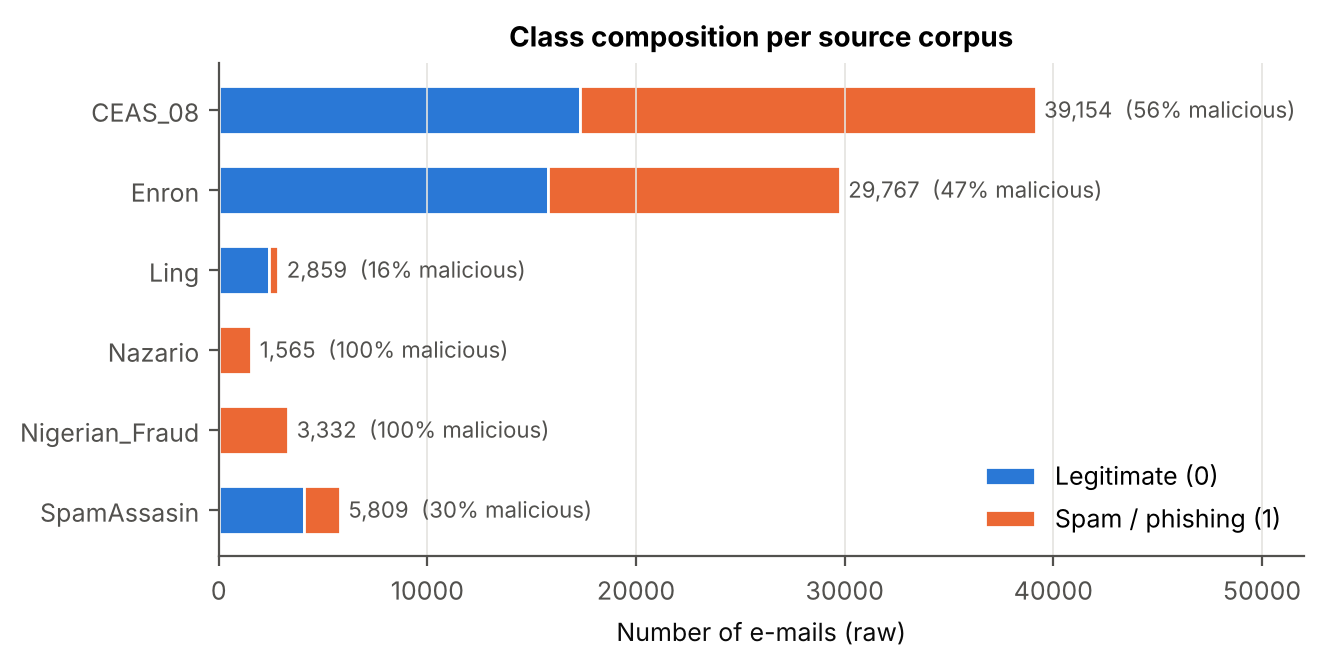
\includegraphics[width=.72\linewidth]{fig1_composition.png}
\caption{Class mix differs strongly between sources: two corpora contain no legitimate e-mail at all.}
\end{figure}

\textbf{Label semantics.} Label 1 means ``spam (phishing)'' in the dataset description: in Enron, Ling, CEAS\_08 and SpamAssassin it is mostly generic spam (pharmacy, dating, stock offers); only Nazario (credential phishing, 2015--2022) and Nigerian\_Fraud (advance-fee scams) are targeted fraud. We therefore frame the task as \emph{malicious/unsolicited vs legitimate}, and use Nazario as a dedicated probe for phishing proper. Using spam corpora for phishing detection is common practice \cite{meajor2025} but must be stated.

\subsection{Missing values}
Missingness is \emph{not at random}: it is decided by the source (Table~\ref{tab:miss}). Enron and Ling have no sender, receiver, date or URL field at all; Nigerian\_Fraud lacks dates for 15\% of rows. Using any metadata feature would therefore encode the source. \textbf{Decision:} only subject + body are used; the 0--2\% missing subjects are replaced by an empty string (the body is never missing).
\begin{table}[H]\centering\small
\caption{Percentage of missing (or empty) values per field and source.}\label{tab:miss}
\tab{tab_missing}
\end{table}

\subsection{Duplicates}\label{sec:dup}
After normalisation (lower-case, punctuation removed) we found 988 exact duplicate copies, 110 groups of them shared between two sources (mostly Enron $\leftrightarrow$ SpamAssassin spam), and no label conflicts.
Near-duplicates were detected with MinHash-LSH \cite{broder1997} (Jaccard $\ge 0.8$ on word 5-shingles, union-find clustering): 13,314 e-mails fall into 3,203 clusters. The four largest (3,919 e-mails, 12\% of CEAS\_08 spam) are the fake ``CNN Alerts: My Custom Alert'' / ``CNN.com Daily Top 10'' messages, a real August-2008 botnet campaign that delivered malware through a fake Flash update \cite{sans2008}, so label 1 is correct, but the campaign is massively over-represented.
\textbf{Decision:} keep one e-mail per near-duplicate cluster (71,386 e-mails left; Table~\ref{tab:comp}). De-duplication is done \emph{before} any split.

\subsection{Outliers and length}
Lengths span five orders of magnitude (Fig.~\ref{fig:len}). A few Nazario e-mails embed base64 attachments (max 4.6M characters); we truncate every e-mail to 20,000 characters (affects $<1.1\%$ of e-mails per source). Length is informative but \emph{inconsistently}: CEAS\_08 spam is much shorter than CEAS\_08 ham, while the opposite holds in SpamAssassin, which is a first hint that per-source patterns may not transfer.
\begin{figure}[H]\centering
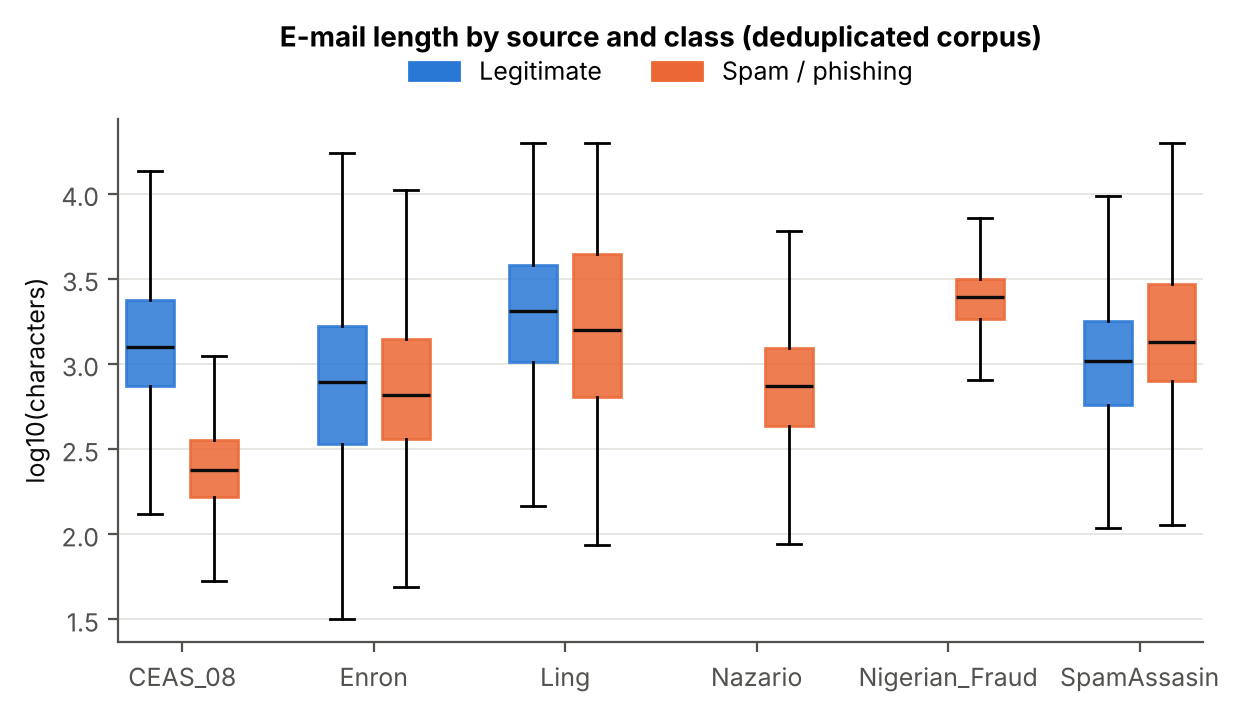
\includegraphics[width=.72\linewidth]{fig2_length.png}
\caption{E-mail length (log scale) by source and class, after de-duplication.}\label{fig:len}
\end{figure}

\subsection{Class imbalance}
The pooled corpus is balanced (47.5\% malicious after dedup), so no re-sampling is needed for training. Imbalance matters in two other places: per source (Ling 15.5\%, SpamAssassin 20.5\%, Nazario/Nigerian 100\%), which drives our split stratification, and at deployment (malicious mail is rare), which is why we report $\mathrm{Prec}_{5\%}$ and FPR instead of accuracy.

\subsection{Source artefacts: the shortcut test}\label{sec:shortcut}
Table~\ref{tab:style} shows that the corpora differ in \emph{form}, independently of intent: Enron and Ling were distributed fully lower-cased and pre-tokenised (``see attached file : hplno 530 . xls''), the other four are raw; collection years range from 2002 to 2022 (Fig.~\ref{fig:years}).
\begin{table}[H]\centering\small
\caption{Style statistics per source (raw text). Years come from the \texttt{date} header.}\label{tab:style}
\begin{adjustbox}{max width=\linewidth}\tab{tab_style}\end{adjustbox}
\end{table}
\begin{figure}[H]\centering
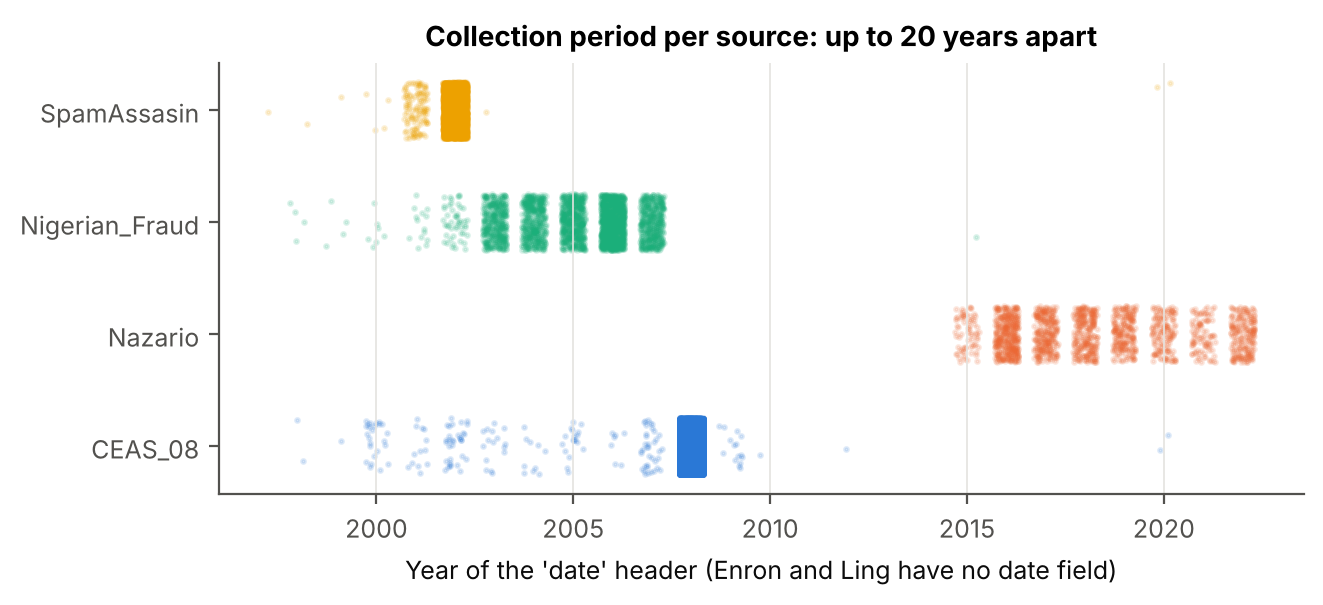
\includegraphics[width=.7\linewidth]{fig4_years.png}
\caption{Collection period per source. Nazario (the only modern phishing corpus) is 8--20 years more recent than the rest.}\label{fig:years}
\end{figure}

To quantify the risk of \emph{shortcut learning} \cite{geirhos2020}, we trained a classifier to predict the \emph{source} from the text (training split, grouped 5-fold CV, linear SVM on TF-IDF).
\begin{table}[H]\centering\small
\caption{How predictable is the source corpus? (chance = majority source)}\label{tab:shortcut}
\tab{tab_shortcut}
\end{table}
Even after our full normalisation, the source is identified 95\% of the time; five style statistics alone reach 85\%. Knowing only the source (no text) already gives 58.2\% label accuracy. Table~\ref{tab:tokens} shows what remains: names (\texttt{vince}, \texttt{kaminski}, \texttt{jose}), host names (\texttt{monkey} = monkey.org, Nazario's mailbox), mailing-list topics (\texttt{opensuse}, \texttt{python}, \texttt{linguistics}) and anonymisation artefacts (\texttt{zzzzteana}). None of them says anything about whether an e-mail is malicious.
\begin{table}[H]\centering\small
\caption{Top source-identifying tokens after cleaning and masking (one-vs-rest linear SVM).}\label{tab:tokens}
\tab{tab_top_tokens}
\end{table}

\subsection{Pre-processing decisions}
\begin{table}[H]\centering\small
\caption{Pre-processing steps and their justification.}
\begin{tabular}{p{0.3\linewidth}p{0.63\linewidth}}
\toprule
Step & Justification (evidence) \\
\midrule
Use per-source files, not the merged CSV & Keeps the source label for LOSO and the shortcut test; avoids undocumented prior transformations. \\
Text = subject + body only & Metadata missing-not-at-random by source (Table~\ref{tab:miss}). \\
Truncate to 20k characters & Base64 attachments up to 4.6M characters; $<1.1\%$ of e-mails affected. \\
Exact + near-duplicate removal before split & 13\% redundancy; one 2008 campaign = 3,919 copies. \\
Lower-case, remove punctuation and underscores & Enron/Ling are lower-cased and tokenised, others are not (Table~\ref{tab:style}). \\
Mask URLs, e-mails, digits (option) & Dates/IDs identify sources (\texttt{2008}, \texttt{713}); URL regex extended to the tokenised form, otherwise masking itself becomes an artefact (AI\_AUDIT \#1). \\
No case/punctuation features & They identify Enron/Ling, not intent. \\
No re-sampling & Pooled classes are balanced; rarity handled in the metrics. \\
\bottomrule
\end{tabular}
\end{table}

%=====================================================================
\section{Learning and testing plan}
\begin{itemize}
\item \textbf{Hold-out test (20\%)}: \texttt{StratifiedGroupKFold}, stratified on source $\times$ label, grouped by near-duplicate cluster, frozen in \texttt{data/processed/split.csv} and used once at the end. Two \texttt{assert}s check that no cluster and no normalised text appears on both sides.
\item \textbf{Model selection}: grouped, stratified $k$-fold CV on the training split only (5 folds for the baseline, 3 for AutoML).
\item \textbf{Out-of-distribution}: LOSO over the six sources. The two positive-only corpora (Nazario, Nigerian\_Fraud) have no negatives, so only recall (detection rate) is defined there, as in \cite{bhuiyan2026}.
\item \textbf{Leakage controls}: dedup before split; every fitted transform (TF-IDF vocabulary and IDF, scaler, $\chi^2$ selector) lives in an \texttt{sklearn} \texttt{Pipeline} refitted inside each fold; source never used as a feature \cite{kapoor2023}.
\item \textbf{Over/under-fitting}: validation curves (train vs validation F1 over the regularisation path) and the train--validation gap logged for every AutoML trial.
\end{itemize}
\begin{table}[H]\centering\small
\caption{Frozen hold-out split.}
\tab{tab_split}
\end{table}

\textbf{Does near-duplicate leakage actually inflate scores?} We tested it on the exact-dedup corpus (near-duplicates kept): random vs grouped split (Table~\ref{tab:infl}). The effect is negligible for this model: near-copies are mostly easy spam that the model gets right either way. We report this null result, and keep the grouped split because it closes the leakage path by construction at no cost.
\begin{table}[H]\centering\small
\caption{Effect of letting near-duplicates cross the split (baseline model).}\label{tab:infl}
\tab{tab_inflation}
\end{table}

%=====================================================================
\section{Baseline}
\textbf{Model.} TF-IDF on unigrams (min\_df = 3, max\_df = 0.95, sublinear TF, 100k features) + L2 logistic regression (liblinear) on the minimally cleaned text. This is the standard text baseline, it is interpretable, and it belongs to the same family as the state-of-the-art reference \cite{bhuiyan2026}, which makes the comparison fair.

\textbf{Calibration of the model.} The only influential hyper-parameter is $C$ (inverse regularisation). Fig.~\ref{fig:vc}: training F1 reaches 1.000 for $C\ge 30$ (memorisation) while validation F1 is flat from $C=10$. The argmax ($C=300$) differs from neighbours by less than one standard error, so we apply the \emph{one-standard-error rule} \cite{esl}: the most regularised $C$ within one SE of the best, i.e.\ $C=30$. The probabilities are well calibrated in-distribution (Brier 0.007, Fig.~\ref{fig:cm}).

\begin{figure}[H]\centering
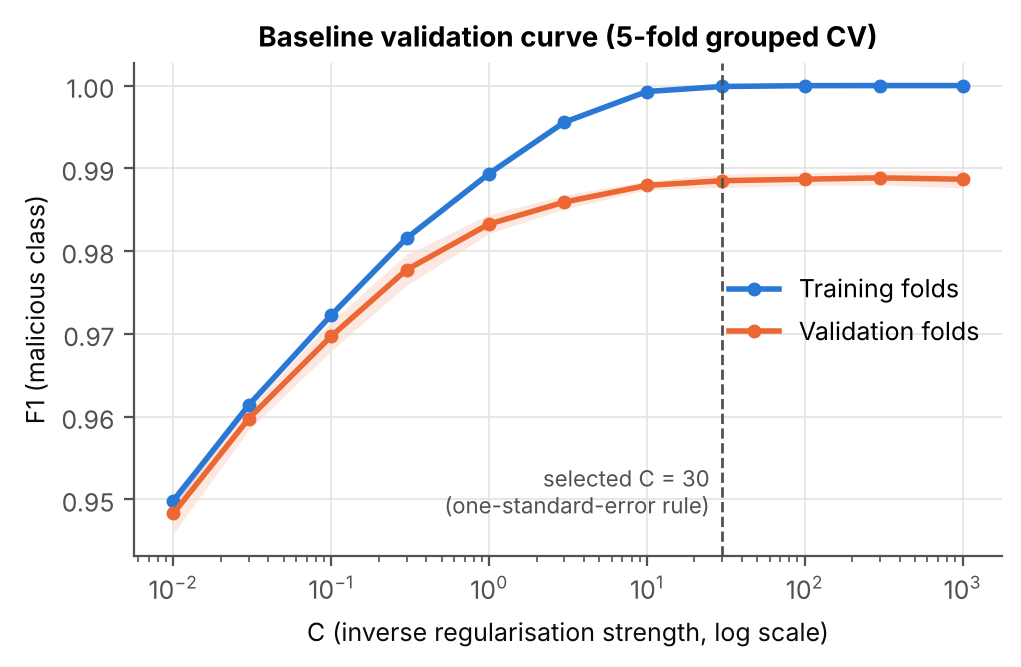
\includegraphics[width=.6\linewidth]{fig5_validation_curve.png}
\caption{Validation curve of the baseline (mean $\pm$ std over 5 grouped folds).}\label{fig:vc}
\end{figure}
\begin{figure}[H]\centering
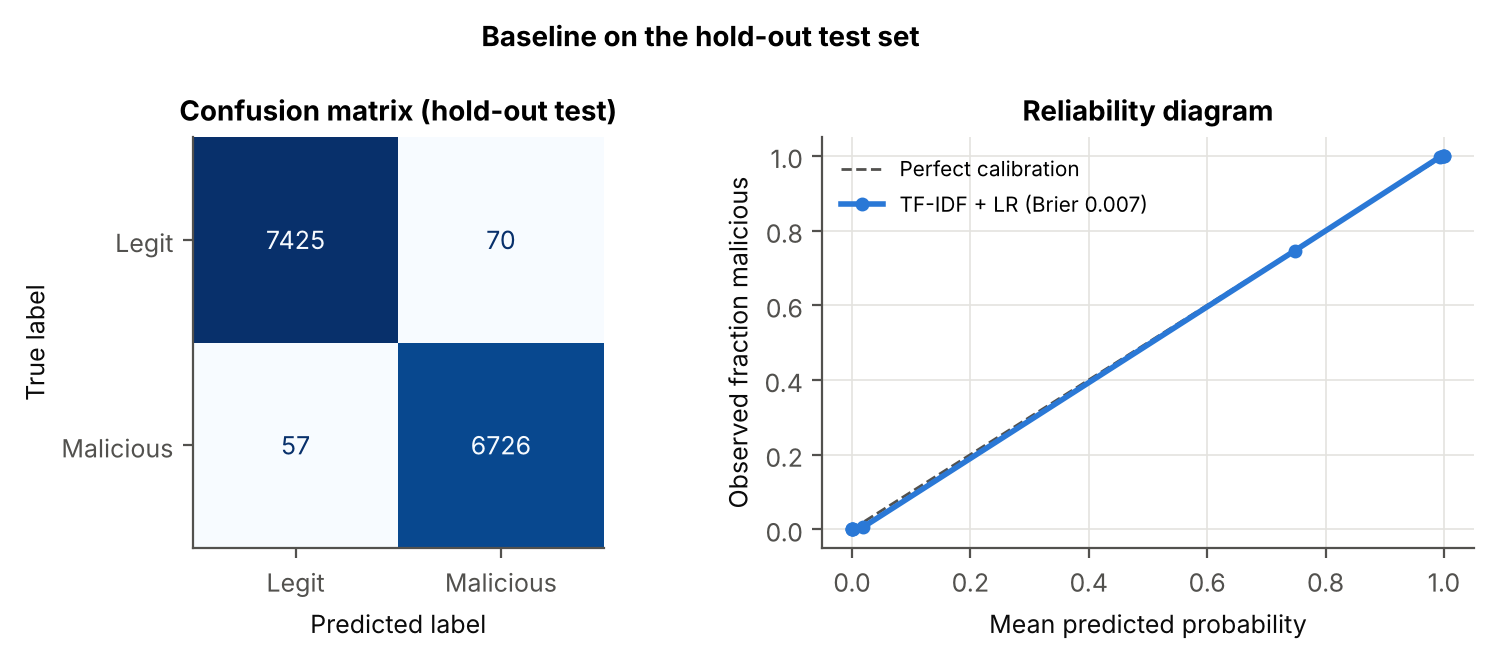
\includegraphics[width=.75\linewidth]{fig6_baseline_cm_calibration.png}
\caption{Baseline on the hold-out test set: confusion matrix and reliability diagram (quantile bins; predictions are very confident, hence few distinct bins).}\label{fig:cm}
\end{figure}

\begin{table}[H]\centering\small
\caption{Baseline on the frozen hold-out test set (14,278 e-mails).}
\tab{tab_baseline}
\end{table}

\textbf{What the baseline learned.} Its strongest coefficients include genuine signals (\texttt{remove}, \texttt{kindly}, \texttt{viagra}, \texttt{urgent}, \texttt{bank}) but also shortcuts: years (\texttt{2004}, \texttt{2005} $\rightarrow$ malicious; \texttt{2008}, \texttt{2002} $\rightarrow$ legitimate), people and hosts (\texttt{jose}, \texttt{monkey} $\rightarrow$ malicious; \texttt{enron}, \texttt{vince}, \texttt{kaminski}, \texttt{713} = Houston area code $\rightarrow$ legitimate). These are invisible in the hold-out score and are exactly what LOSO exposes.

\textbf{Out-of-distribution.}
\begin{table}[H]\centering\small
\caption{Baseline in-distribution vs leave-one-source-out, compared with the LOCO results of Bhuiyan \& Bhuiyan (2026, Tables 18--19, TF-IDF + LR).}\label{tab:loso}
\begin{adjustbox}{max width=\linewidth}\tab{tab_loso}\end{adjustbox}
\end{table}
\begin{figure}[H]\centering
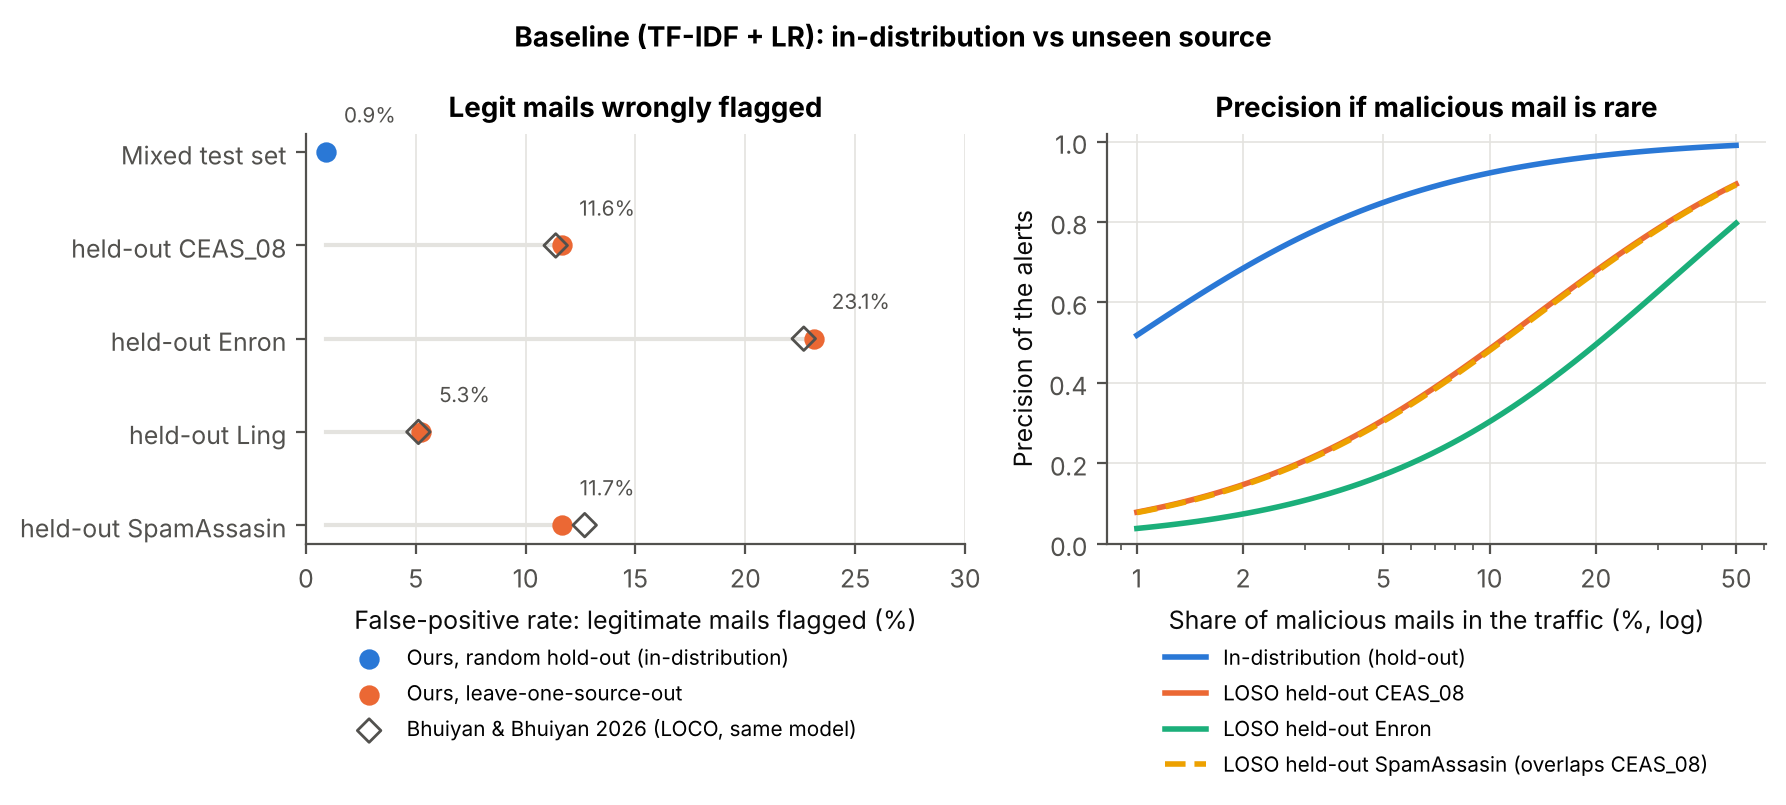
\includegraphics[width=.92\linewidth]{fig7_generalisation_gap.png}
\caption{Left: false-positive rate in-distribution vs on an unseen source. Right: precision of the alerts as a function of the share of malicious mail in the traffic.}\label{fig:gap}
\end{figure}
Three findings: (1) the F1 drops from 0.991 to 0.80--0.94 and the FPR is multiplied by 6 to 25 (Fig.~\ref{fig:gap}); at a realistic 5\% prevalence, fewer than one alert in three would be a true threat on CEAS\_08, Enron or SpamAssassin; (2) only 59\% of the modern Nazario phishing e-mails are caught when Nazario is unseen, a temporal and topical shift, not a class-balance issue, since 98--99\% of the older Nigerian scams are still detected; (3) our independent pipeline reproduces the published LOCO numbers (FPR within 1.1 points on all four corpora), which validates our protocol.

%=====================================================================
\section{State-of-the-art benchmarks}
\begin{table}[H]\centering\small
\caption{Published results on this dataset. In-distribution scores are saturated; the honest benchmark for our question is the LOCO one.}
\begin{adjustbox}{max width=\linewidth}
\begin{tabular}{p{3.6cm}p{4.1cm}p{3.7cm}p{3.6cm}}
\toprule
Reference & Model & Protocol & Reported result \\
\midrule
Al-Subaiey et al.\ 2024 \cite{alsubaiey2024} (dataset authors) & TF-IDF + linear SVM & 80/20 random split of the merged CSV, no source-level analysis & Acc.\ 0.991, F1 0.99 \\
Ahmed \& Pourmoafi 2026 \cite{ahmed2026} & TF-IDF (1--2 g, 20k) + LR; DistilBERT & 80/20 stratified random split; external IWSPA adversarial set & F1 0.986 (LR), 0.991 (DistilBERT); adversarial accuracy drops by $\approx$35 points for both \\
Bhuiyan \& Bhuiyan 2026 \cite{bhuiyan2026} & TF-IDF (unigrams, 5k) + LR / linear SVC & Leave-one-corpus-out; source-prediction test & LOCO F1 0.82--0.90 (LR); source predictable at 97.2\% \\
\midrule
\textbf{Ours (baseline)} & TF-IDF (unigrams, 100k) + LR, $C$ by 1-SE rule & Dedup + grouped split; LOSO & F1 0.991 hold-out; LOSO F1 0.80--0.94; Nazario recall 0.59 \\
\bottomrule
\end{tabular}
\end{adjustbox}
\end{table}
None of the three papers reports de-duplication. Our contribution relative to \cite{bhuiyan2026}, whose protocol we adopt and reproduce, is planned in Section~\ref{sec:plan}: artefact-removal ablations, model families beyond linear TF-IDF, and selection criteria aligned with the out-of-distribution goal.

%=====================================================================
\section{AutoML pipeline v0.1}\label{sec:automl}
\textbf{Pipeline.} One \texttt{sklearn} pipeline per configuration:
\emph{data preparation} (minimal cleaning vs masking) $\rightarrow$
\emph{feature engineering} (word TF-IDF; optional character 3--5-gram TF-IDF; optional hand-crafted, source-agnostic statistics: log length, number of URLs/e-mail addresses, digit density, ``!'' and currency density, count of urgency words, all scaled with MaxAbsScaler) $\rightarrow$
\emph{feature selection} ($\chi^2$, keep 100\%/50\%/20\%) $\rightarrow$
\emph{model selection} (logistic regression, linear SVM, complement naive Bayes \cite{rennie2003}, SGD with modified Huber loss, ridge least-squares classifier, i.e.\ linear regression on $\{-1,+1\}$ targets, decision tree) $\rightarrow$
\emph{hyper-parameter optimisation} (Optuna TPE sampler with median pruning \cite{optuna}). The same \texttt{build\_features()} object is used in the search and in the final refit.

\textbf{Search protocol.} Stratified subsample of 20,000 training e-mails, 3-fold grouped CV, objective = mean validation F1, Optuna TPE sampler (seed 42) with median pruning. Each family is seeded with one default configuration so that all six are evaluated at least once.

\textbf{What actually happened (reported as is).} Run~1 used the same $C$ range for logistic regression and linear SVM ($10^{-2}$--$10^{3}$) and had no time budget. Linear-SVM trials at large $C$ did not converge and took over 200\,s each, so we aborted it (AI\_AUDIT \#6). Run~2 capped the SVM at $C\le 100$ and added a 25-minute budget, but it was stopped manually after \IfFileExists{tables/val_automl.tex}{\nTrials{} trials (\nComplete{} completed, \nPruned{} pruned)}{34 trials}, before its refit phase, to keep the week's compute bounded. The search log only stores scores, so we recovered the exact parameters by \emph{replaying} the deterministic sampler on the logged history (\path{scripts/05b_recover_best.py}). We then \emph{re-computed} the CV score of the top configurations: all reproduce their logged score to four decimals. Three configurations tie at CV F1 = 0.9827. We keep the \IfFileExists{tables/val_automl.tex}{\bestFamily{} (trial \bestTrial)}{ridge least-squares} configuration, as recorded in the log, and saved it in \path{reports/tables/automl_best_config.json}:
\IfFileExists{tables/val_automl_cfg.tex}{\begin{center}\smallmasked, word 1--2-grams, min\_df=5, 100k features, + char 3--5-grams, no stats, no selection, $\alpha$=0.0442\end{center}}{}

\IfFileExists{tables/tab_automl_best.tex}{
\begin{table}[H]\centering\small
\caption{Search summary per model family (CV F1 on the training subsample).}\label{tab:automlfam}
\tab{tab_automl_families}
\end{table}
\begin{table}[H]\centering\small
\caption{Baseline vs AutoML v0.1 best configuration, both refitted on the full training split. Same hold-out test and LOSO protocol.}\label{tab:automl}
\tab{tab_automl_best}
\end{table}
\begin{figure}[H]\centering
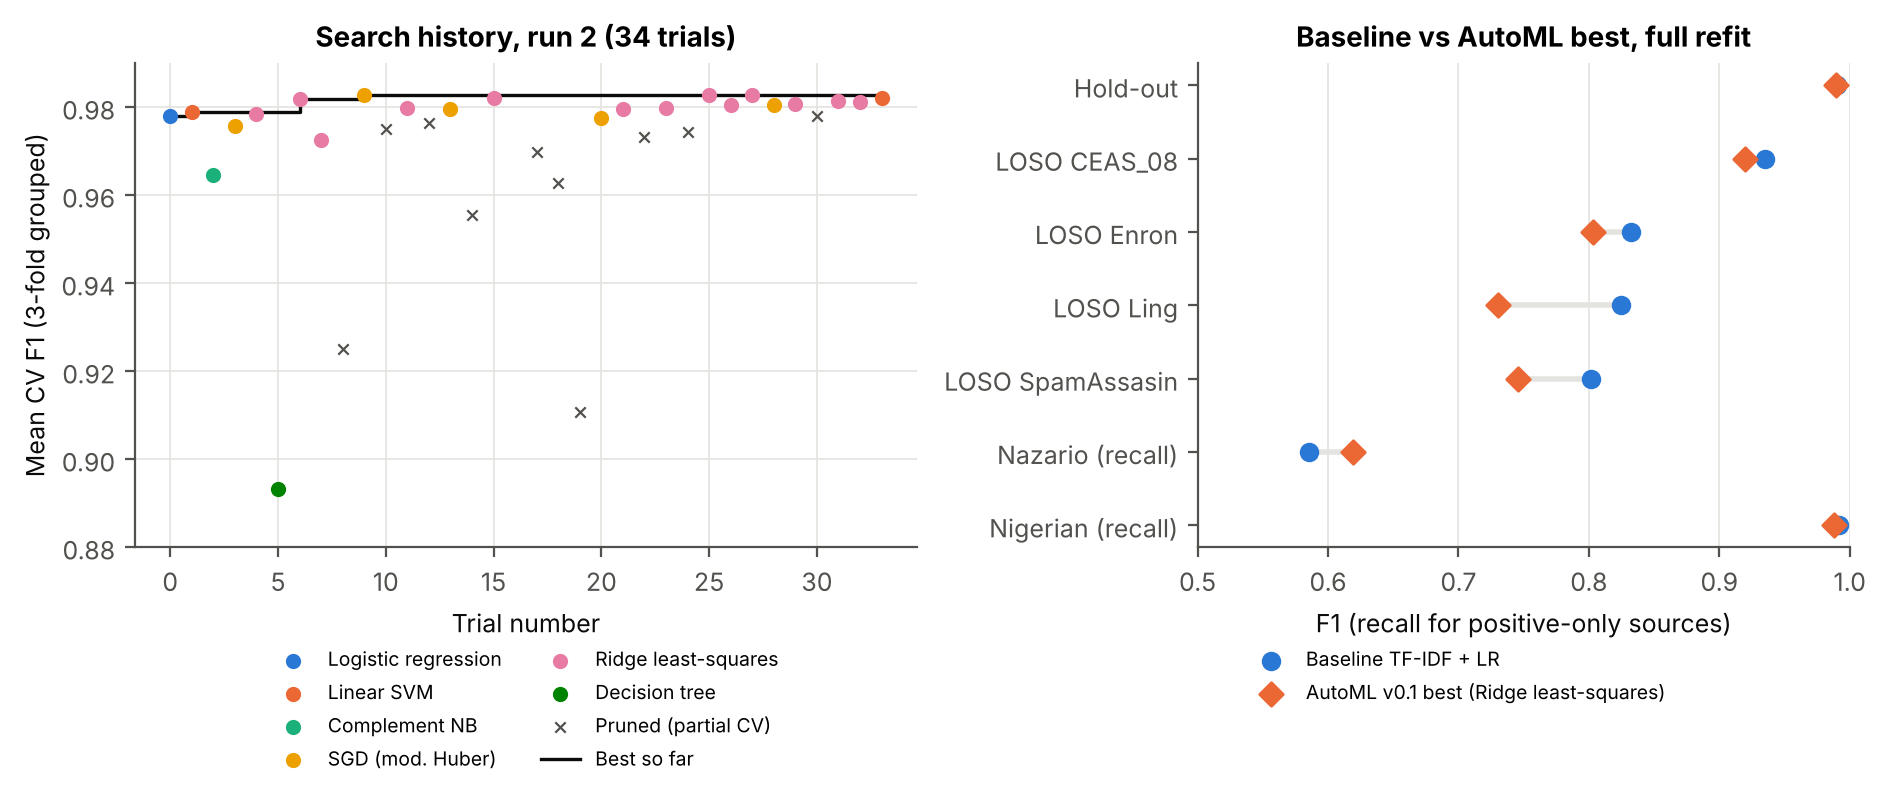
\includegraphics[width=.95\linewidth]{fig8_automl.png}
\caption{Left: search history of run 2. Right: baseline vs AutoML best configuration, in-distribution and per unseen source.}\label{fig:automl}
\end{figure}
\textbf{Reading the results.}
\begin{itemize}
\item \textbf{The search space is flat at the top.} Five of six families reach a CV F1 within 0.005 of each other (Table~\ref{tab:automlfam}). The single decision tree is far behind (0.89): one tree cannot exploit 100k sparse, weakly informative features. Three configurations tie at 0.9827, and the default logistic regression of the search (0.9779) is only half a point of F1 below, on a 20k subsample.
\item \textbf{In-distribution, AutoML trades a little recall for fewer false positives.} On the hold-out test, the selected ridge model has a lower FPR (0.65\% vs 0.93\%) and therefore a better precision at 5\% prevalence (0.888 vs 0.848), for a slightly lower F1 (0.989 vs 0.991).
\item \textbf{Out-of-distribution, AutoML is worse on three of the four binary sources.} F1 drops on CEAS\_08 ($-0.015$), Enron ($-0.030$), Ling ($-0.094$) and SpamAssassin ($-0.055$). FPR improves on CEAS\_08 and Enron but worsens on Ling and SpamAssassin. Only the Nazario recall improves (0.619 vs 0.585). The selected model is \emph{more complex} (word bigrams + character 3--5-grams, 150k features, weak regularisation $\alpha=0.044$, training F1 = 1.000): it fits the training sources better, including their artefacts, and transfers worse.
\item \textbf{Conclusion for v0.1.} Optimising an in-distribution objective selects for memorisation of source-specific patterns. This is direct empirical evidence that the selection criterion, not the model family, is the bottleneck. It makes nested LOSO selection (Section~\ref{sec:plan}) the first priority.
\end{itemize}

}{\todo{AutoML results}}

%=====================================================================
\section{Evaluation protocol, risks and plan}\label{sec:plan}
\textbf{Evaluation protocol (fixed for all future versions).} Frozen grouped hold-out for in-distribution scores; LOSO for out-of-distribution scores (full metrics on CEAS\_08, Enron, Ling, SpamAssassin; recall on Nazario and Nigerian\_Fraud); headline metrics FPR, recall, F1 and $\mathrm{Prec}_{5\%}$; every new model compared with the baseline under both regimes.

\textbf{Risks and failure modes.}
\begin{itemize}
\item \emph{Shortcut learning}: the model relies on names, years, hosts and formatting (Section~\ref{sec:shortcut}). Monitored via top coefficients and the source-prediction test.
\item \emph{Selection leakage across sources}: AutoML v0.1 selects on in-distribution CV, so the chosen configuration has seen every source; its LOSO scores are slightly optimistic.
\item \emph{Label semantics}: label 1 is mostly spam; conclusions about \emph{phishing} must rely on the Nazario probe.
\item \emph{Temporal drift}: training data is 2000--2008 for the most part; modern phishing (Nazario) is under-detected.
\item \emph{Threshold}: 0.5 is not the right operating point under prevalence shift; FPR must be controlled explicitly.
\item \emph{Residual near-duplicates} below Jaccard 0.8 and remaining label noise (spam vs ham boundaries differ between corpora).
\end{itemize}

\textbf{Prioritised plan (v0.2 $\rightarrow$ v0.4).}
\begin{enumerate}
\item \textbf{Nested LOSO model selection}: select hyper-parameters on the training sources only (inner leave-one-source-out), so that LOSO scores become unbiased and selection rewards transfer instead of memorisation. \emph{(Highest priority: Section~\ref{sec:automl} shows that in-distribution selection picks a model that transfers worse.)} Persist every trial (Optuna SQLite storage) so that a stopped search loses nothing.
\item \textbf{Artefact ablation}: block-list of source-identifying tokens (names, hosts, list tags, years) and measure the change in LOSO FPR; repeat the source-prediction test after ablation.
\item \textbf{Operating point}: choose the threshold for a target FPR (e.g.\ 1\%) on validation sources; report recall at fixed FPR.
\item \textbf{Ensembles} (course scope): soft voting / stacking of the best linear models + gradient boosting on dense features.
\item \textbf{Out-of-course model}: fine-tuned DistilBERT, motivated by \cite{ahmed2026}; question: does a pretrained language model rely less on corpus artefacts and transfer better to Nazario?
\item \textbf{Fresh test set}: a small set of recent real phishing e-mails from our own inboxes (anonymised) as a final sanity check.
\end{enumerate}

%=====================================================================
\section*{AI usage}
Claude (Anthropic) was used as an engineering accelerator for boilerplate code, EDA drafting and literature search, following the course policy. Critical prompts are logged in \path{ai-governance/PROMPT_LOG.md}; six concrete flaws in AI-generated ML logic that we caught and corrected (e.g.\ a masking regex that silently created a new source artefact, an invalid 6-fold LOSO plan, a hyper-parameter chosen at the grid boundary, a search space that made the linear SVM diverge) are documented in \path{ai-governance/AI_AUDIT.md}. Every number in this report is produced by \texttt{run\_all.sh}; tables are generated from result files (\texttt{scripts/07\_latex\_tables.py}).

\begin{thebibliography}{99}\small
\bibitem{bhuiyan2026} I.~Bhuiyan and T.~Bhuiyan. The fragility of phishing detection models: evidence from cross-corpus transfer, prevalence shift, artifact learning, and evasion risk. \emph{Big Data and Cognitive Computing}, 10(7):211, 2026. doi:10.3390/bdcc10070211.
\bibitem{alsubaiey2024} A.~Al-Subaiey, M.~Al-Thani, N.~A.~Alam, K.~F.~Antora, A.~Khandakar, S.~M.~A.~U.~Zaman. Novel interpretable and robust web-based AI platform for phishing email detection. \emph{Computers and Electrical Engineering}, 2024. arXiv:2405.11619.
\bibitem{ahmed2026} T.~Ahmed and S.~Pourmoafi. Adversarial robustness of phishing email detection: a comparative study of TF-IDF + logistic regression and fine-tuned DistilBERT. arXiv:2607.18429, 2026.
\bibitem{champa_zenodo} A.~I.~Champa, M.~F.~Rabbi, M.~F.~Zibran. Phishing Email Curated Datasets. Zenodo, record 8339691 (CC-BY-4.0).
\bibitem{meajor2025} P.~Mendes, E.~Maia, et al. MeAJOR Corpus: a multi-source dataset for phishing email detection. arXiv:2507.17978, 2025.
\bibitem{sans2008} SANS Internet Storm Center. ``CNN -- My Custom Alert'', diary 4841, 8 August 2008. \url{https://isc.sans.edu/diary/4841}.
\bibitem{broder1997} A.~Z.~Broder. On the resemblance and containment of documents. \emph{Compression and Complexity of Sequences}, IEEE, 1997.
\bibitem{geirhos2020} R.~Geirhos et al. Shortcut learning in deep neural networks. \emph{Nature Machine Intelligence}, 2:665--673, 2020.
\bibitem{kapoor2023} S.~Kapoor and A.~Narayanan. Leakage and the reproducibility crisis in machine-learning-based science. \emph{Patterns}, 4(9), 2023.
\bibitem{esl} T.~Hastie, R.~Tibshirani, J.~Friedman. \emph{The Elements of Statistical Learning}, 2nd ed., Springer, 2009 (Sec.~7.10, one-standard-error rule).
\bibitem{rennie2003} J.~D.~M.~Rennie, L.~Shih, J.~Teevan, D.~R.~Karger. Tackling the poor assumptions of naive Bayes text classifiers. \emph{ICML}, 2003.
\bibitem{optuna} T.~Akiba, S.~Sano, T.~Yanase, T.~Ohta, M.~Koyama. Optuna: a next-generation hyperparameter optimization framework. \emph{KDD}, 2019.
\bibitem{ruta2025} Ruta et al. ChatGPT for univariate statistics: validation of AI-assisted data analysis in healthcare research. \emph{Journal of Medical Internet Research}, 2025.
\end{thebibliography}

\appendix
\section*{Appendix: missing-value map}
\begin{figure}[H]\centering
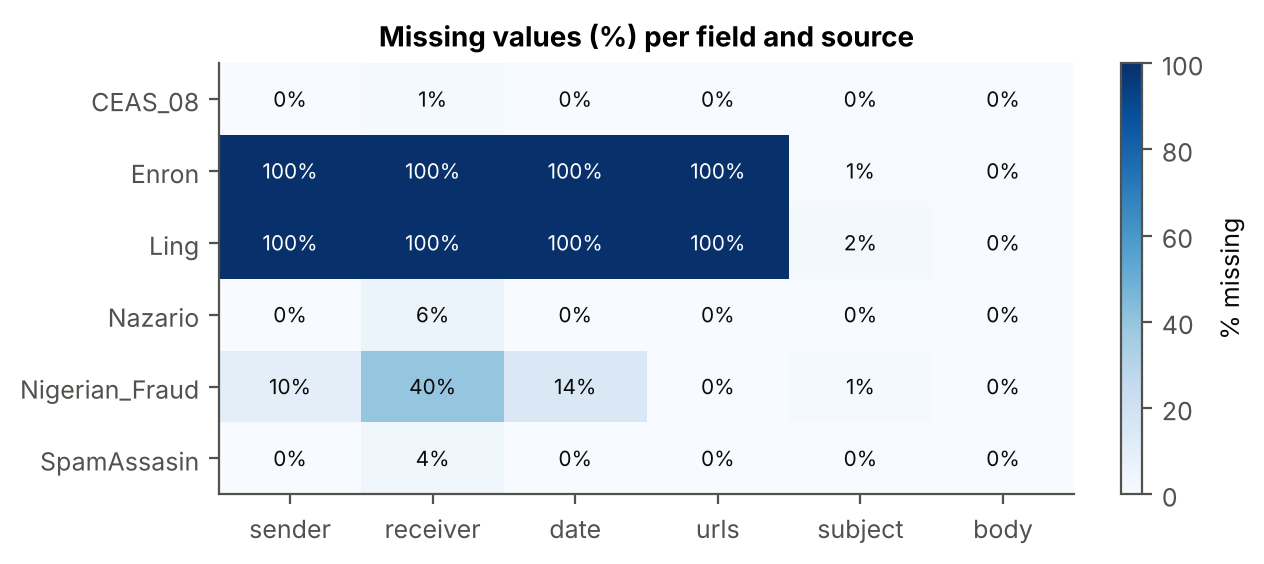
\includegraphics[width=.6\linewidth]{fig3_missingness.png}
\caption{Missing values per field and source: metadata availability is entirely determined by the source.}
\end{figure}
\end{document}
